\documentclass[12pt]{extarticle}
\usepackage{preamble}

\begin{document}
\thispagestyle{empty}

\begin{tikzpicture}[remember picture,overlay]
   \node[xshift=6.5cm,yshift=-2cm] at (current page.north west)
              {
\includegraphics[scale= 1]{banner.pdf}};
\end{tikzpicture}

\bigskip

% TITLE
%------------------------------------------------------
{\fontfamily{qtm}\selectfont
\color{titlecolor}
\centerline{\huge{\textbf{Title}}}
%\centerline{\LARGE{\textbf{long_title1}}}
%\centerline{\LARGE{\textbf{long_title2}}} 
\bigskip
\centerline{\Large{\textbf{Subtitle}}}
}

\bigskip
\bigskip

\centerline{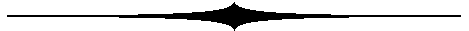
\includegraphics[scale=0.25]{divider}}

\bigskip
\bigskip

% AUTHOR NAME
%------------------------------------------------------
% leave blank for peer review copy
\centerline{ \large AUTHOR NAME\footnotemark}

\bigskip

\centerline{ date-here }

% BIO
%------------------------------------------------------
% leave blank for peer review copy
\footnotetext{Author info}

\bigskip
\bigskip

% ABSTRACT
%------------------------------------------------------
\noindent \textbf{Abstract}

Your abstract here.

\bigskip

\textbf{Keywords}: key; words

\bigskip

\textbf{Citation}:

suggested-citation

\bigskip
\bigskip

% licence
%------------------------------------------------------
\begin{centering}
	
\vfill


\includegraphics[scale=0.5]{by-nc-nd} \vspace{-0.8em}

\footnotesize
\href{commons-link}{CC BY-NC-ND 4.0}

\vfill

\end{centering}


\newpage
% begin content
%------------------------------------------------------

\section{Introduction}

\lettrine[lines=3,lraise=0.1, nindent=0em]{F}{irst} word \lipsum[1]


\lipsum[1]

\section{Methods}
\lipsum[1]

% EQUATION
\begin{equation}
K = \frac{E}{r}
\end{equation}

% FIGURE WITH CAPTION AND NOTES
\begin{figure}
	\centerline{
\includegraphics[scale=0.15]{fig_142.png}}
	\caption{Differential capitalization and differential net profit in the United States}
	\label{fig_diff_capital}
	
	\small
	\smallskip
	
	This figure is from \cite{nitzan_capital_2009}. \\
	
	 * Ratio between the average market capitalization of the top 100 Compustat corporations (ranked annually by market capitalization) and the average market capitalization of all US listed corporations. \\
	
	** Ratio between the average net profit of the top 100 Compustat corporations (ranked annually by market capitalization) and the average net profit of all US corporations (listed and unlisted). The number of US corporations for 2004–2006 is extrapolated based on recent growth rates. \\
	
	Source: Compustat compann file through WRDS (series codes: data25 for common shares outstanding; data199 for share price; data172 for net income); Global Financial Data (number of listed corporations on the NYSE, AMEX and NASDAQ till 1989); World Federation of Exchanges (number of listed corporations on the NYSE, AMEX and NASDAQ from 1990); U.S. Internal Revenue Service (number of corporate tax returns for active corporations); U.S. Federal Reserve Board’s Flow of Funds through Global Insight (FL893064105 for market value of corporate equities); U.S. Bureau of Economic Analysis through Global Insight (ZA for profit after taxes).	
	
\end{figure}

% REFERENCE YOUR FIGURE
This is a reference to Figure \ref{fig_diff_capital}, which shows the differential capitalization and net profit of dominant capital in the United States.




\section{Discussion}
\lipsum[1]

% A BLOCK QUOTE
\begin{quote}
\lipsum[1]
\end{quote}

\section{Conclusions}
\lipsum[1]


\newpage
% BIBLIOGRAPHY
% either compile with bibtex and paste your bbl contents below,
% or uncomment \bibliography{bib_file} and enter your bib file
%\bibliography{your_bib}{}

\begin{thebibliography}{6}
	\providecommand{\natexlab}[1]{#1}
	\expandafter\ifx\csname urlstyle\endcsname\relax
	\providecommand{\doi}[1]{doi:\discretionary{}{}{}#1}\else
	\providecommand{\doi}{doi:\discretionary{}{}{}\begingroup
		\urlstyle{rm}\Url}\fi
	
	\bibitem[{Baines(2014)}]{baines_food_2014}
	Baines, Joseph. 2014.
	\newblock Food price inflation as redistribution: towards a new analysis of
	corporate power in the world food system.
	\newblock \emph{New Political Economy} 19(1):79--112.
	
	\bibitem[{Cochrane(2010)}]{cochrane_death_2010}
	Cochrane, D.T. 2010.
	\newblock Death Grip: Scapegoating the Subprime Loser.
	\newblock \emph{SCAPEGOAT Architecture/ Landscape/Political Economy} (00):6--8.
	
	\bibitem[{Fix(2015)}]{fix_putting_2015}
	Fix, Blair. 2015.
	\newblock Putting Power Back into Growth Theory.
	\newblock \emph{Review of Capital as Power} 1(2):1--37.
	
	\bibitem[{Hager(2014)}]{hager_what_2014}
	Hager, Sandy~Brian. 2014.
	\newblock What happened to the bondholding class? Public debt, power and the
	top one per cent.
	\newblock \emph{New Political Economy} 19(2):155--182.
	
	\bibitem[{McMahon(2018)}]{mcmahon_is_2018}
	McMahon, James. 2018.
	\newblock Is {Hollywood} a Risky Business? A Political Economic Analysis of
	Risk and Creativity.
	\newblock \emph{New Political Economy} :1--23.
	
	\bibitem[{Nitzan and Bichler(2009)}]{nitzan_capital_2009}
	Nitzan, Jonathan and Bichler, Shimshon. 2009.
	\newblock \emph{Capital as Power: A Study of Order and Creorder}.
	\newblock New York: Routledge.
	
\end{thebibliography}

\end{document}
